\documentclass[twoside,11pt]{article}

% Any additional packages needed should be included after jmlr2e.
% Note that jmlr2e.sty includes epsfig, amssymb, natbib and graphicx,
% and defines many common macros, such as 'proof' and 'example'.
%
% It also sets the bibliographystyle to plainnat; for more information on
% natbib citation styles, see the natbib documentation, a copy of which
% is archived at http://www.jmlr.org/format/natbib.pdf

\usepackage{jmlr2e}
\usepackage{xcolor}

% Definitions of handy macros can go here

\newcommand{\dataset}{{\cal D}}
\newcommand{\fracpartial}[2]{\frac{\partial #1}{\partial  #2}}
\newcommand{\todo}{\textcolor{red}}

% Heading arguments are {volume}{year}{pages}{date submitted}{date published}{paper id}{author-full-names}

%\jmlrheading{1}{2018}{1-48}{4/00}{10/00}{meila00a}{Przemyslaw Biecek}
%\ShortHeadings{DALEX: explainers for complex predictive models}{Przemyslaw Biecek}

\usepackage{lastpage}
\jmlrheading{19}{2018}{1-\pageref{LastPage}}{6/18; Revised
10/18}{11/18}{18-416}{Przemyslaw Biecek}
\ShortHeadings{DALEX: Explainers for Complex Predictive Models in R}{Biecek}

% Short headings should be running head and authors last names

\firstpageno{1}


\begin{document}

\title{DALEX: Explainers for Complex Predictive Models in R}

\author{\name Przemys\l{}aw Biecek \email przemyslaw.biecek@gmail.com \\
       \addr Faculty of Mathematics and Information Science, Warsaw University of Technology\\
       75 Koszykowa Street, Warsaw, Poland\\
       Samsung Research Poland}


\editor{Alexandre Gramfort}

\maketitle

\begin{abstract}%   <- trailing '%' for backward compatibility of .sty file
Predictive modeling is invaded by elastic, yet complex methods such as neural networks or ensembles (model stacking, boosting or bagging). Such methods are usually described by a large number of parameters or hyper parameters - a price that one needs to pay for elasticity. The very number  of parameters makes models hard to understand. 

This paper describes a consistent collection of explainers for predictive models, a.k.a. black boxes. Each explainer is a technique for exploration of a black box model. Presented approaches are model-agnostic, what means that they extract useful information from any predictive method irrespective of its internal structure. Each explainer is linked with a~specific aspect of a model. Some are useful in decomposing predictions, some serve better in understanding performance, while others are useful in understanding importance and conditional responses of a particular variable.

Every explainer presented here works for a single model or for a collection of models. In the latter case, models can be compared against each other. Such comparison helps to find strengths and weaknesses of different models and gives additional tools for model validation. Presented explainers are implemented in the \texttt{DALEX} package for R. They are based on a~uniform standardized grammar of model exploration which may be easily extended. 
\end{abstract}

\begin{keywords}
interpretable machine learning, explainable artificial intelligence, predictive modelling, model visualization \end{keywords}

\section{Introduction}

Predictive modeling has a large number of applications in almost every area of human activity, starting from medicine, marketing, logistic, banking and many others. Due to the increasing amount of collected data, models become more sophisticated and complex. 

It is believed that there is a trade-off between the interpretability and accuracy of a~model \citep[see][]{tradeoff_interpretability_accuracy}. It comes from the observation that the most elastic models usually have higher accuracy but in turn they are also more complex. Complexity here means a large number of model parameters that affect the final prediction. That number is big enough to make the model ununderstandable for an ordinary human being.

In many areas we cannot sacrifice interpretability, either because of legal requirements (see  \textit{right to explanation} in GDPR), or because it leads to unfair decisions \citep[see][]{ONeil} or because it is important for users \citep[see][]{shapley}. Interpretability brings multiple benefits such as:
 a) helps to extract interpretable patterns from trained models; b) helps to identify reasons behind poor predictions; c) increases trust in model predictions \citep[see][]{lime}; d) reduces the hidden debt in machine learning models \citep[see][]{Dennison_2015}; e) helps to detect bias in machine learning models; f) creates additional safety catch that may protect from overfitted models. 
 
In this paper we present a consistent general framework for exploration of black-box models. This framework covers the most known approaches to interpretability and structure exploration, such as Partial Dependence Plots \citep{pdp}, Accumulated Local Effects Plots \citep{ALEPlot}, Merging Path Plots \citep{factorMerger}, Break Down Plots \citep{breakDownlive}, Permutational Variable Importance Plots \citep{Fisher2018} or Cateris Paribus Plots. An unique feature of \texttt{DALEX} explainers is that they can be natively used to compare two or more models. Model comparison helps to understand differences in model responses, gives new insights that may be used to construct new, better features. 

Presented framework is available as an open source package \texttt{DALEX} for R. The R language \citep{Rcran} is one of the most popular languages for statistical and machine learning modeling. \texttt{DALEX} works with any predictive model. The extended user documentation\footnote{User documentation is available at \url{https://pbiecek.github.io/DALEX\_docs}.} contains examples for the most popular frameworks, such as \texttt{caret} \citep{caret}, \texttt{mlr} \citep{mlr}, Random Forest and Gradient Boosting Machines. 
The \texttt{DALEX} package is available on at CRAN and GitHub\footnote{Development version is available at \url{https://github.com/pbiecek/DALEX}.} along with technical documentation\footnote{Technical documentation is available at \url{https://pbiecek.github.io/DALEX}.}.

Example explainers presented in this paper were recorded with the \texttt{archivist} package \citep{archivist}. To save space, we present only graphical explainers. Numerical explainers can be downloaded with R commands listed in footnotes. 

\section{Architecture}
Figure \ref{fig:architecture} presents the general architecture of the \texttt{DALEX} package. This methodology is model-agnostic and works for predictive models, such as classification or regression models. 

Methods for understanding of global structure of a model (a.k.a. model explainers) and for  understanding of a local structure of a model (a.k.a. prediction explainers) are implemented in separate functions. We call these functions \textit{explainers} since they are designed to explain a single feature of a model. Every explainer returns numerical summaries in a~tabular format. These tables may be visualized with generic \texttt{plot} function. The \texttt{plot} function works also for multiple models and overlays model explainers in a single chart. See examples in Figure 1 panels F, I and J. 


\subsection{Prediction Understanding: Explainers for Variable Attribution}

The most known approaches to explanations of a single prediction are \textit{LIME} method \citep{lime},  for local variable importance, and \textit{Shapley values} \citep{shapley}, for local variable attribution. \textit{Break Down Plots} are fast approximations of \textit{Shapley values}. Comparison of these methods is presented in \citet{breakDownlive}.
An example for these explainers\footnote{Access this explainer with \texttt{archivist::aread('pbiecek/DALEX\_arepo/72b47')}.} is presented in Figure 1 panels C and D. 

Note, that for non additive models, the local model behaviour may be very different from global model behaviour. Consider $f(x_1, x_2) = x_1*x_2$ around point $(0, 0)$.


\begin{figure}[tb]
\centering
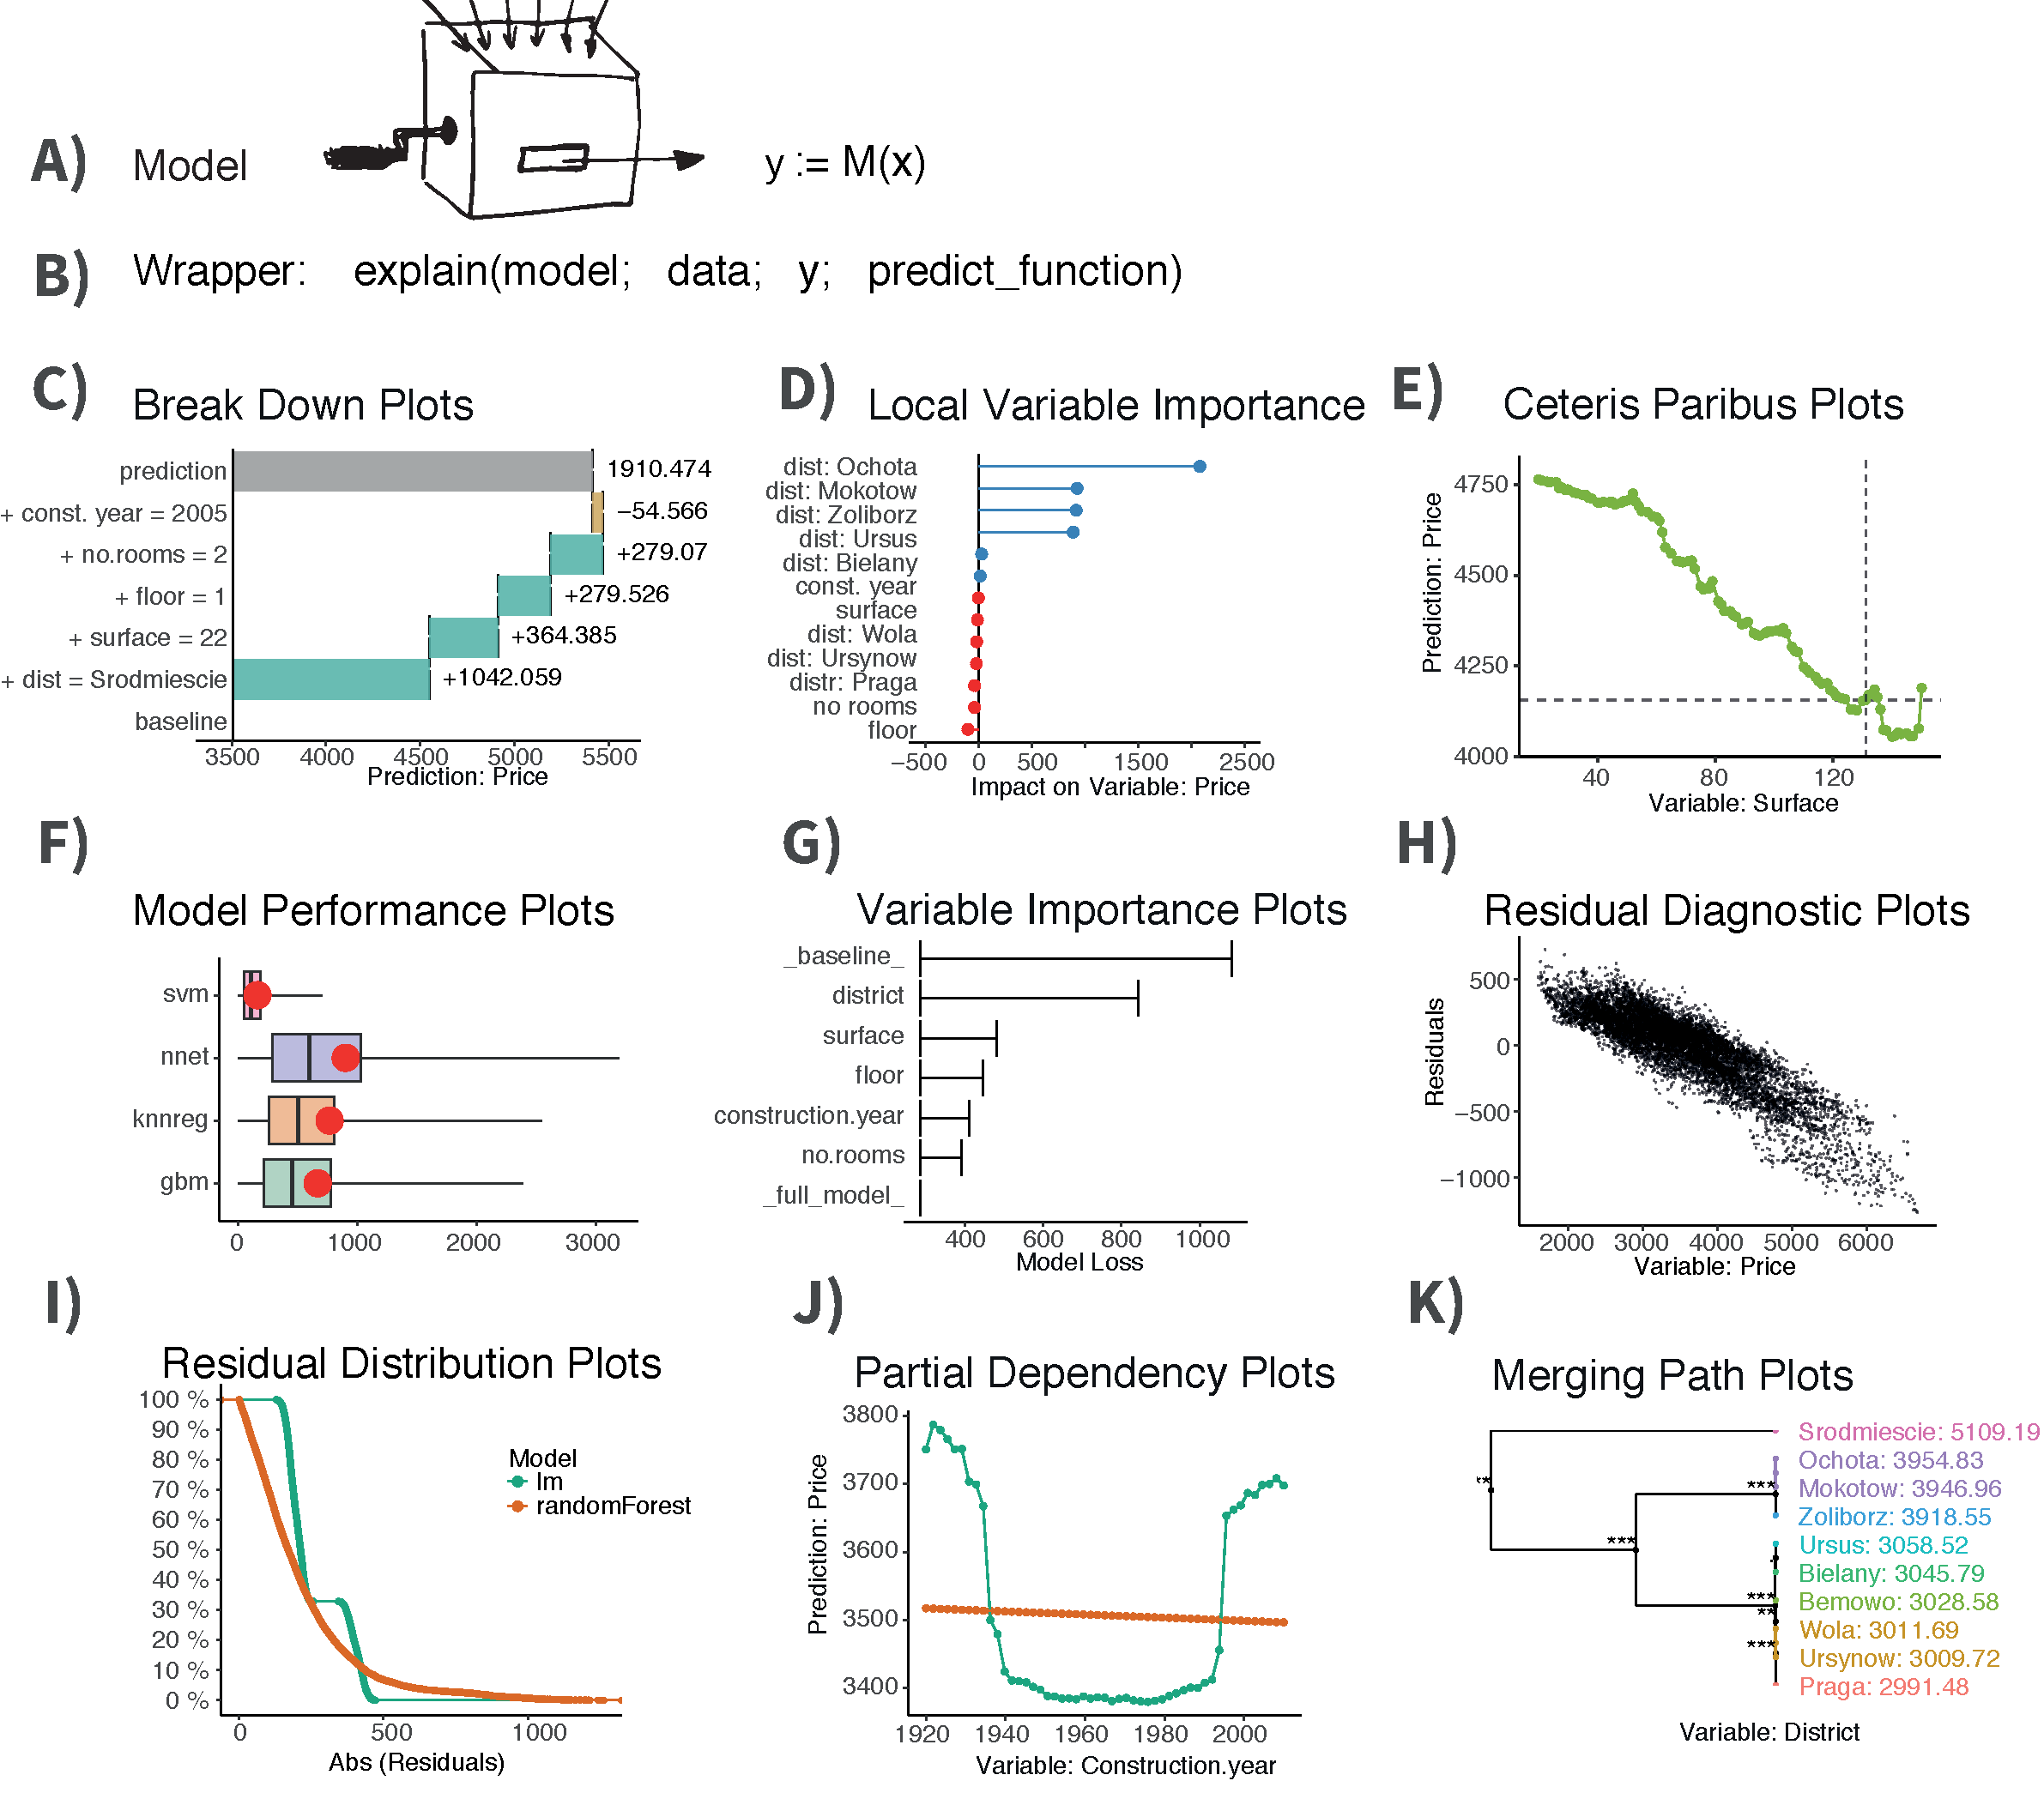
\includegraphics[width=0.95\textwidth]{architecture1.pdf}
\caption{\label{fig:architecture}Architecture of the \texttt{DALEX} package is based on simple  unified grammar. A)~Any predictive model $M: \mathcal R^p \rightarrow \mathcal R$ may be used. B) Models are first enriched with additional metadata with the function \texttt{explain()}. Each explainer returns numerical summaries that can be plotted with generic \texttt{plot()} function. C, D, E) Explainers for a single prediction. F) Comparison of four models. G, H) Explainers for a single model, I) Comparison of residuals for two models. J, K) Explainers for a single variable, respectively continuous and categorical.}
\end{figure}


\subsection{Prediction Understanding: Explainers for What-If Scenarios}

\textit{Ceteris Paribus Profiles} show how the model response changes as a function of a single variable. These plots recollect similarities to more known \textit{Partial Dependency Plots}. The difference between them is that \textit{Ceteris Paribus Profiles} are focused on a single observation.

An example for this explainer\footnote{Access this explainer with \texttt{archivist::aread('pbiecek/DALEX\_arepo/c8989')}.}, is presented in Figure 1 panel E. One can read how model response will change for an altered value of a~single variable.%created with  \texttt{ceterisParibus} package

\subsection{Model Understanding: Explainers for Model Performance}

Model performance is often summarized with a single number such as \textit{F1} or \textit{accuracy}. %Such approach is handy in model selection. 
This makes it easier to construct a ranking of models and choose the best one. However, more descriptive statistics are better when it comes to understanding of a model. The descriptive statistics most often used for classification is \textit{ROC (Receiver Operating Characteristic)} with various extensions for regression as in \cite{RROC}. 
% It has many various implementations. In R, the most widely used descriptive statistic is the \texttt{ROCR} package \cite{ROCR}. ROC plots have also extensions for regression models. 

The \texttt{DALEX} package offers a selection of tools for exploration of model performance, see Figure 1 panels F and I\footnote{Access this explainer with  \texttt{archivist::aread('pbiecek/DALEX\_arepo/b4eb1')}.}, and model diagnostic, see Figure 1 panel H.
The latter is available through the \texttt{auditor} package \citep{auditor}, closely integrated with \texttt{DALEX}. 



\subsection{Model Understanding: Explainers for Effect of a Single Variable}
\label{sec:pdpexpl}

The \texttt{DALEX} package offers a selection of tools for better understanding of a  conditional model's response based on a single variable. 
For continues variables it supports \textit{Partial Dependence Plot} \citep{pdp} as implemented in the \texttt{pdp} package and  \textit{Accumulated Local Effects Plot} \citep{ALEPlot} as implemented in \texttt{ALEPlot} package, see Figure 1 panel~J\footnote{Access this explainer with  \texttt{archivist::aread('pbiecek/DALEX\_arepo/3b150')}.}.
For categorical variables it supports \textit{Merging Path Plot} \citep{factorMerger} as implemented in the \texttt{factorMerger} package. See Figure 1 panel K.

\subsection{Model Understanding: Explainers for Variable Importance}

The \texttt{DALEX} package offers a model-agnostic procedure to calculate variable importance. The model-agnostic approach is based on permutational approach introduced initially for \textit{Random Forest} \citep{Breiman2001} and then extended for other models by \cite{Fisher2018}.

An example for these explainers\footnote{Access this explainer with \texttt{archivist::aread('pbiecek/DALEX\_arepo/9378c')}.} is presented in Figure 1 panel G. It's common in variable importance charts to hitch bars in 0. 
Charts in the \texttt{DALEX} package present not only drop in model performance but also the initial model performance. In that way one can compare variables between models with different initial performance.


\section{Summary}


In this article we have introduced consistent methodology and tools for model-agnostic explanations. Global explainers (for model understanding) and local explainers (for prediction understanding) are based on uniform grammar. Every explainer creates a numerical summary, visual summary and allows for comparison of multiple models. The \texttt{DALEX} package is tested with CI tools and is easy to extend\footnote{Extended version of this paper is available at \url{https://arxiv.org/pdf/1806.08915v1.pdf}.}. Here we presented \texttt{DALEX}  0.2.5 with \texttt{R} 3.5.1.

\acks

The work was financially supported by RENOIR Project under the Marie Sk\l odowska-Curie grant agreement No 691152 and NCN Opus grant 2016/21/B/ST6/02176.

\setlength{\bibsep}{4pt plus 0.3ex}

\vskip 0.2in
\bibliography{18-416}

\end{document}

